\section{Entanglement Entropy II}

\subsection{Review of Entanglement entropy}
Given $\rho = \dyad{\psi}{\psi}$, we can partition the set of qubits which $\rho$ lives on into two subsets $A, A^c$. We can then define the Von Neumann entanglement entropy:
\begin{equation}
    S(\rho_A) = -\Tr(\rho_A\log \rho_A)
\end{equation}
with $\rho_A$ the reduced density operator:
\begin{equation}
    \rho_A = \Tr_{A^c}(\rho)
\end{equation}
this has some nice properties:
\begin{enumerate}
    \item $S(\rho_A) = S(\rho_{A^c}) = -\sum_i \abs{\lambda_i}^2\log(\abs{\lambda_i}^2)$ with $\lambda_i$ the Schmidt coefficients discussed last class.
    \item $S$ measures entanglement between $A, A^c$, with $S(\rho_A) = 0 \iff \ket{\psi} = \ket{\psi_A} \otimes \ket{\psi_B}$. Conversely, $S(\rho_A) \neq 0 \iff \ket{\psi} \text{is entangled}$.
\end{enumerate}

The absolute simplest example is for the Bell pair, or singlet state:
\begin{equation}
    \ket{\psi} = \frac{1}{\sqrt{2}}(\ket{\uparrow}_A\otimes \ket{\downarrow}_{A_c} - \ket{\downarrow}_A \otimes \ket{\downarrow}_{A_c})
\end{equation}
This is basically already written in terms of a Schmidt decomposition, just need to make the coefficients positive:
\begin{equation}
    \ket{\psi} = \frac{1}{\sqrt{2}}\ket{\uparrow}_A \otimes \ket{\downarrow}_{A^c} + \frac{1}{\sqrt{2}}\ket{\downarrow}_A \otimes (-\ket{\uparrow}_{A^c})
\end{equation}
so $\lambda_1 = \lambda_2 = \frac{1}{\sqrt{2}}$. The entanglement entropy is thus:
\begin{equation}
    S(\rho_A) = \log(2)
\end{equation}
in information theory the convention of base-2 logarithms is often used, but let us just write things using the natural log here. Roughly, we can think of $S(\rho_A)$ to be measuring the number of Bell pairs that are shared across $A$ and $A^c$.

\subsection{Scaling of entanglement entropy in gapped ground states}
The setting has been thus far for very general quantum systems. Now, we ask about the entanglement properties of ground states of local Hamiltonians. The best understood case is gapped ground states, which we will talk about now. 

Let $\ket{\psi}$ be the unique ground state of a gapped finite-range Hamiltonian $H$ defined on an infinite $d$-dimensional lattice. Let $A$ be a finite subset:

\begin{center}
    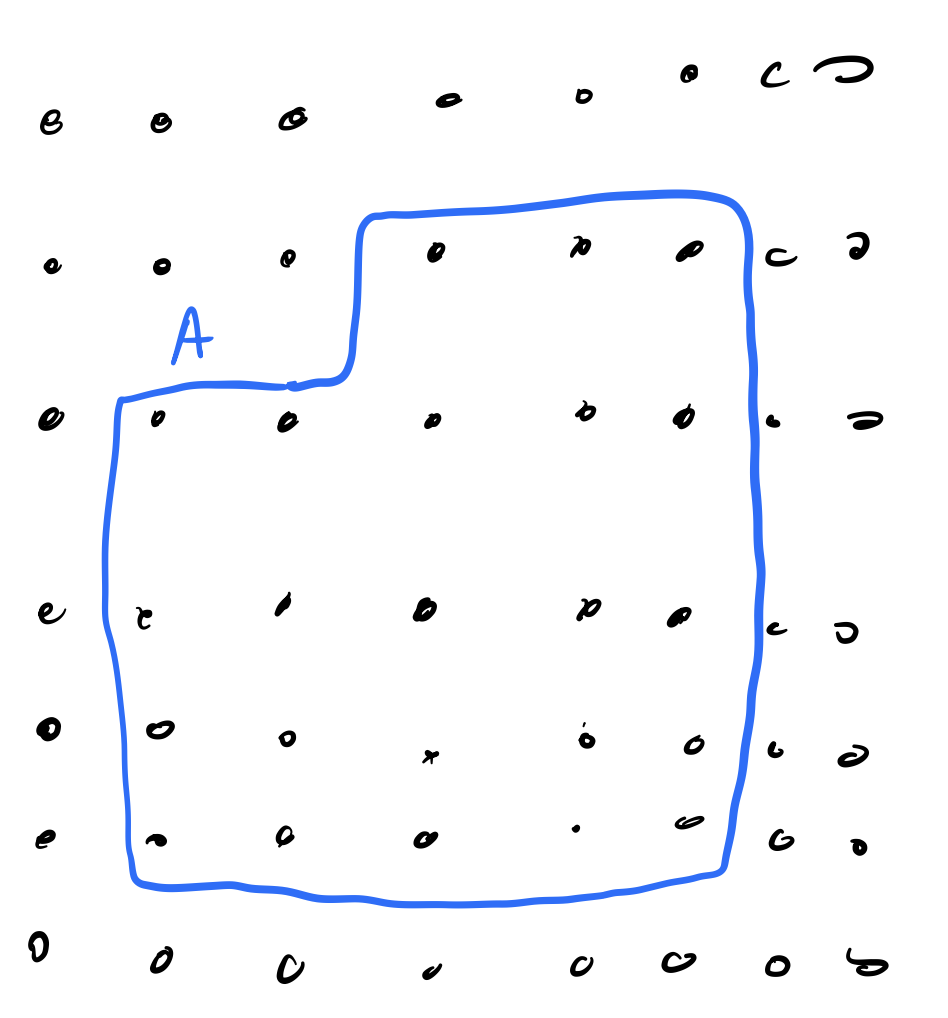
\includegraphics[scale=0.35]{Lectures/Images/lec16-Aregion.png}
\end{center}

The most basic question we can ask is how does $S(\rho_A)$ scale with $A$? This is not just a curiosity, but also has some practical implications - the scaling can have implications for ease of classical simulation.

This is generically a difficult question to answer. It has not been answered except in some special cases. But there is a hand-wavey intuition for what the answer should be, as well as many examples where it has been calculated.

The intuition proceeds as follows. Gapped states have short-range correlations (follows from Lieb-Robinson bounds; we also saw it during the discussion of anyons). More precisely:
\begin{equation}
    \bra{\psi}O_1O_2\ket{\psi} = \bra{\psi}O_1\ket{\psi}\bra{\psi}O_2\ket{\psi} + \text{exponentially small quantity in $\text{dist}(O_1, O_2)$}
\end{equation}
We could equivalently say this as the connected correlator:
\begin{equation}
    \avg{O_1O_2}_c = \avg{O_1O_2} - \avg{O_1}\avg{O_2}
\end{equation}
is exponentially small in the distance between $O_1, O_2$. In a rough sense, there is an exponential supression of singlets across long distances. There is only singlets/entangelment on short distances.

Hence - we expect (handwavey jump) that only degrees of freedom near the boundary of $A$ are entangled with $A^c$.

\begin{center}
    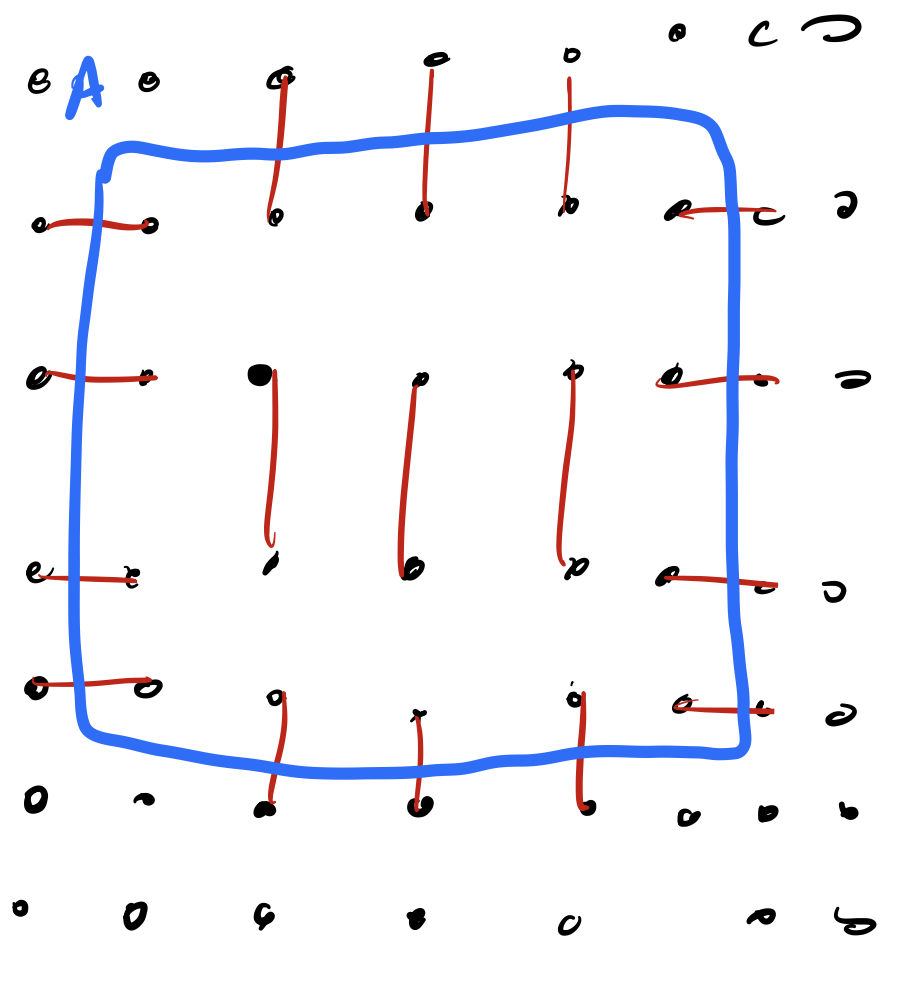
\includegraphics[scale=0.35]{Lectures/Images/lec16-perimeterlaw.png}
\end{center}

So we thus expect that $S(\rho_A) \propto \text{length/area}$ of the boundary. We call this ``area law'' scaling (coming from 3D; the boundary of a volume has an area).

Question - can an operation on one subset change the entanglement across the boundary? Sometimes we use the probe of mutual information which is monotonic under local operations $I(A:B) = S(\rho_A) + S(rho_B) - S(\rho_{AB})$ which for pure states is just $2S(\rho_A)$.

\subsection{Area law conjecture}
\emph{Area law conjecture.} If $\ket{\psi}$ is the unique gapped ground state of a finite range Hamiltonian $H$, then:
\begin{equation}
    S(\rho_A) \leq C\abs{\p A}
\end{equation}
Where $\abs{\p A}$ is the number of edges o the lattice that connect $A, A^c$, i.e. the length/area of the boundary of $A$. $C$ is some constant that depends only on $\ket{\psi}$, not on $A$.

A few comments about this inequality:
\begin{enumerate}
    \item The maximum possible value of $S(\rho_A) = \abs{A}\log(\dim(\mathcal{H}_{site}))$, e.g. $N\log(2)$ for a region of $N$ qubits, for example. This maximum follows from the Schmidt decomposition; the maximum number of Schmidt states we could have is $\dim(\mathcal{H}_A) = \dim(\mathcal{H}_{\text{site}})^{\abs{A}}$, and the maximum entropy we could have is the logarithm of this. Pictorially, the maximum entanglement is for each site in $A$ to be entangled with something on the outside. In other words, the entanglement scales with the \emph{volume} of $A$. A comment about this - if we choose a random pure state in the Hilbert space (say we truncated the lattice so this is a meaningful statement). Then, with probability 1, we would find that the state is volume law entangled. In other words, typical states in Hilbert space are highly entangled. Thus, gapped ground states are very different from random states. This is good, because random states are somewhat hopeless to try to describe classically - there is thus some hope for classical simulation of ground states of interest.
    \item In 1D systems (for a bipartition $A, A^c$), the area law conjecture reduces to:
    \begin{equation}
        S(\rho_A) \leq C
    \end{equation}
    since the boundary is just a point ($\abs{\p A} = \mathcal{O}(1)$). This has been proven rigorously for nearest-neighbour interaction, with:
    \begin{equation}
        C = \mathcal{O}(\frac{\log^3\dim(\mathcal{H}_{\text{site}})}{\Delta}).
    \end{equation}
    This bound is proven in (Arad, Kitaev, Landau, Vazirani \texttt{1301.1162}).
    \item In higher dimensions, the conjecture is unproven. There are some partial results in 2D frustration-free system; models for which the ground state is an eigenstate of individual terms of the Hamiltonian (Anshu, \texttt{2103.02492}). Nevertheless, it is widely believed to be true.
\end{enumerate}

\subsection{Scaling of entanglement entropy in 1D gapless states}
Consider an infinite 1D chain. Let $\ket{\psi}$ be the ground state of a finite range \emph{gapless} Hamiltonian $H$ whose low energy properties are described by a (1+1)D ``conformal field theory'' (most gapless systems are). Some properties of CFTs:
\begin{enumerate}
    \item Spacetime correlation functions $\avg{O_1(x_1, t_1)O_2(x_2, t_2)\ldots}$ are scale invariant and Lorentz invariant with respect to some velocity $v$.
    \item When defined on a finite system, all low-lying eigenstates have energies $E \propto \frac{1}{L}$ with $L$ the system size.
\end{enumerate}
An example is the transverse field Ising model (TFIM) tuned to the critical point. The TFIM Hamiltonian is:
\begin{equation}
    H = -\sum_i Z_i Z_{i+1} - h\sum_i X_i
\end{equation}
with a phase transition from the ferromagnetic/ordered phase to the paramagnetic/disordered phase at $h = 1$, which is where we have a CFT.

\begin{center}
    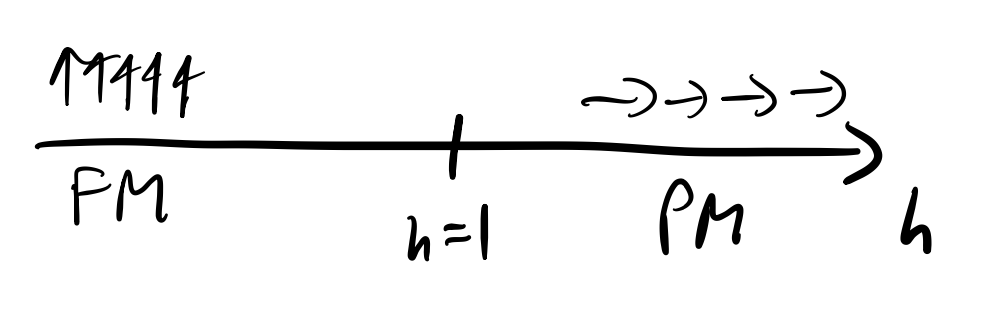
\includegraphics[scale=0.35]{Lectures/Images/lec16-TFIMphases.png}
\end{center}

Consider an interval $A$ of length $l$. Now we can ask the question; how does $S(\rho_a)$ scale with $l$?

\begin{center}
    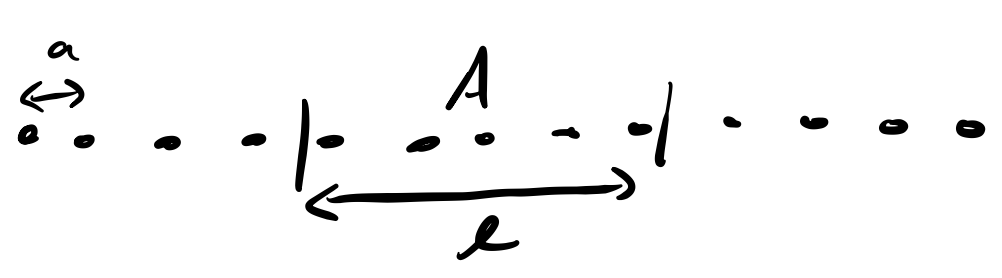
\includegraphics[scale=0.35]{Lectures/Images/lec16-CFT.png}
\end{center}

The answer is beautiful (and so is the derivation, though we don't have time to discuss here). The answer is:
\begin{equation}
    S(\rho_A) = \frac{c}{3}\log(\frac{l}{a}) + \mathcal{O}(1)
\end{equation}
with $c$ the central charge of the CFT. It is a real number that characterizes the number of low energy degrees of freedom.

Another number which characterizes the low energy DoFs is the low temperature specific heat of the CFT. Indeed, this is likely the historical origin for why we use $c$. It indeed the case that:
\begin{equation}
    \text{specific heat} \sim \frac{\pi}{3}cT
\end{equation}
(though there is also a velocity-dependent term, so the above is quite loose). For example, $c = \frac{1}{2}$ for the TFIM. 

The upshot - the entanglement entropy gives us a beautiful way to directly probe/measure (e.g. in numerics) the central charge of a CFT, even if we can't solve the model. For details, see (Cardy and Calabrese \texttt{0905.4013}). 

For our last lecture, we will discuss topological entanglement entropy.